\documentclass[a4paper, 11pt]{article}           %{{{1
% basic packages                                  {{{2
\usepackage[T1]{fontenc}
\usepackage[scaled=0.975]{helvet}
\usepackage[utf8]{inputenc}
\usepackage{amsmath}
\usepackage{lastpage}
\usepackage{graphicx}
\usepackage{amsfonts}
\usepackage{variations}
\usepackage{pgf,tikz}           % dessin
\usepackage{mathrsfs}
\usetikzlibrary{arrows}
\usepackage{pgfkeys}        % fenetrage des plot TikZ
\usepackage{yhmath}         % arc au dessus des lettres
\usepackage{calc}           % calcul de longueur
\usepackage{variations}     % tableau de variations
\usepackage{multicol}
\usepackage{enumitem}
% ==== PROGRAMMATION
\usepackage{xcolor}                                                             %
\usepackage{listings}                                                           %
% listings                                        {{{3
\definecolor{mygreen}{rgb}{0,0.6,0}
\definecolor{mygray}{rgb}{0.5,0.5,0.5}
\definecolor{mymauve}{rgb}{0.58,0,0.82}
\definecolor{deepblue}{rgb}{0,0,0.5}
\definecolor{deepred}{rgb}{0.6,0,0}
\definecolor{deepgreen}{rgb}{0,0.5,0}
\lstset{%
%       backgroundcolor=\color{white},   % choose the background color; you must add \usepackage{color} or \usepackage{xcolor}; should come as last argument
        basicstyle=\footnotesize,        % the size of the fonts that are used for the code
%       breakatwhitespace=false,         % sets if automatic breaks should only happen at whitespace
%       breaklines=true,                 % sets automatic line breaking
%       captionpos=b,                    % sets the caption-position to bottom
        commentstyle=\color{mygreen},    % comment style
%       deletekeywords={type},           % if you want to delete keywords from the given language
%       emph={},                         % Custom highlighting
%       emphstyle=\ttb\color{deepred}    % Custom highlighting style
%       escapeinside={\%*}{*)},          % if you want to add LaTeX within your code
%       extendedchars=true,              % lets you use non-ASCII characters; for 8-bits encodings only, does not work with UTF-8
        frame=shadowbox,                 % adds a frame around the code {single, shadowbox}
%       keepspaces=true,                 % keeps spaces in text, useful for keeping indentation of code (possibly needs columns=flexible)
        keywordstyle=\color{blue},       % keyword style
	language=Python,                 % the language of the code {Python, C}
%       morekeywords={*,...},            % if you want to add more keywords to the set
        numbers=left,                    % numbers = (none, left, right)
%       numbersep=5pt,                   % how far the line-numbers are from the code
%       numberstyle=\tiny\color{mygray}, % the style that is used for the line-numbers
%       otherkeywords={self},            % Add keywords here
%       rulecolor=\color{black},         % if not set, the frame-color may be changed on line-breaks within not-black text (e.g. comments (green here))
	rulesepcolor=\color{gray}        % shadowbox color
%       showspaces=false,                % show spaces everywhere adding particular underscores; it overrides 'showstringspaces'
%       showstringspaces=false,          % underline spaces within strings only
%       showtabs=false,                  % show tabs within strings adding particular underscores
%       stepnumber=1,                    % the step between two line-numbers. If it's 1, each line will be numbered
%       stringstyle=\color{mymauve},     % string literal style
%       tabsize=4,                       % sets default tabsize to 2 spaces
%       title=\lstname                   % show the filename of files included with \lstinputlisting; also try caption instead of title
}
%}}}
%}}}

% mise en page                                    {{{2
\addtolength{\voffset}{-1.8cm}
\addtolength{\textheight}{4cm}
\addtolength{\hoffset}{-2.5cm}
\addtolength{\textwidth}{4cm}
\addtolength{\headsep}{-0.5cm}
\usepackage{fancyhdr}
\setlength{\headheight}{14.00pt}
\pagestyle{fancy} % Numérotation des pages
\renewcommand\headrulewidth{1pt}
\fancyhead[L]{BP SN}
\fancyhead[C]{micro:bit}
\fancyhead[R]{introduction}
\renewcommand\footrulewidth{1pt}
\fancyfoot[L]{v 1.1 -- J.B.}
\fancyfoot[C]{\textbf{domotique, syst. embarqués \& de gestion de l'habitat}}
\fancyfoot[R]{\thepage/\pageref{LastPage}}
%\lhead{3E}%haut de page gauche
%}}}

% Compteurs:                                     {{{2
\addtocounter{page}{0}
\newcounter{Q}
\newcounter{exoNB}
%}}}

% Longueur:                                      {{{2
\newlength{\longueurA}
\newlength{\longueurB}
\setlength{\parindent}{0pt}
\setlength{\parskip}{2pt}
\renewcommand{\baselinestretch}{1}
%}}}

% newcommand                                     {{{2
\newcommand{\objectif}[1]{\textsc{\huge #1} }
\newcommand{\partie}[1]{\textsc{\huge #1} }
\newcommand{\question}{\stepcounter{Q} $\boxed{\arabic{Q}}$ }
\newcommand{\ligne}{\underline{\hspace{ \textwidth}} }
\newcommand{\LIGNE}{\vspace{2mm}\underline{\hspace{ \textwidth}} }
\newcommand{\reponse}{
  \par\nobreak
  \noindent\rule{0pt}{1.5\baselineskip}% Provides a larger gap between the preceding paragraph and the dots
  {\noindent\makebox[\linewidth]{\dotfill}\endgraf}% ... dotted lines ...
% \bigskip% Gap between dots and next paragraph
  }
\newcommand{\exo}[1]{\stepcounter{exoNB}\textsc{\Large Exercice \arabic{exoNB} -- #1} }
\newcommand{\EXO}[2]{\stepcounter{exoNB}\textsc{\Large Exercice \arabic{exoNB} -- #1} \hfill \textbf{#2 points}}
\newcommand{\pb}[1] {\stepcounter{exoNB}\textsc{\Large Problème \arabic{exoNB} -- #1} }
\newcommand{\PB}[2] {\stepcounter{exoNB}\textsc{\Large Problème \arabic{exoNB} -- #1} \hfill \textbf{#2 points}}
%}}}

% Divers                                          {{{2
% listings                                        {{{3
%\definecolor{mygreen}{rgb}{0,0.6,0}
%\definecolor{mygray}{rgb}{0.5,0.5,0.5}
%\definecolor{mymauve}{rgb}{0.58,0,0.82}
%\definecolor{deepblue}{rgb}{0,0,0.5}
%\definecolor{deepred}{rgb}{0.6,0,0}
%\definecolor{deepgreen}{rgb}{0,0.5,0}
%\lstset{%
%        backgroundcolor=\color{white},   % choose the background color; you must add \usepackage{color} or \usepackage{xcolor}; should come as last argument
%        basicstyle=\footnotesize,        % the size of the fonts that are used for the code
%        breakatwhitespace=false,         % sets if automatic breaks should only happen at whitespace
%        breaklines=true,                 % sets automatic line breaking
%        captionpos=b,                    % sets the caption-position to bottom
%        commentstyle=\color{mygreen},    % comment style
%        deletekeywords={...},            % if you want to delete keywords from the given language
%        escapeinside={\%*}{*)},          % if you want to add LaTeX within your code
%        extendedchars=true,              % lets you use non-ASCII characters; for 8-bits encodings only, does not work with UTF-8
%        frame=single,                    % adds a frame around the code
%        keepspaces=true,                 % keeps spaces in text, useful for keeping indentation of code (possibly needs columns=flexible)
%        keywordstyle=\color{blue},       % keyword style
%        morekeywords={*,...},            % if you want to add more keywords to the set
%        numbers=left,                    % where to put the line-numbers; possible values are (none, left, right)
%        numbersep=5pt,                   % how far the line-numbers are from the code
%        numberstyle=\tiny\color{mygray}, % the style that is used for the line-numbers
%        rulecolor=\color{black},         % if not set, the frame-color may be changed on line-breaks within not-black text (e.g. comments (green here))
%        showspaces=false,                % show spaces everywhere adding particular underscores; it overrides 'showstringspaces'
%        showstringspaces=false,          % underline spaces within strings only
%        showtabs=false,                  % show tabs within strings adding particular underscores
%        stepnumber=2,                    % the step between two line-numbers. If it's 1, each line will be numbered
%        stringstyle=\color{mymauve},     % string literal style
%        tabsize=4,                       % sets default tabsize to 2 spaces
%        title=\lstname                   % show the filename of files included with \lstinputlisting; also try caption instead of title
%}
%\lstset{%
%        language=Python,                 % the language of the code
%        otherkeywords={self},            % Add keywords here
%        deletekeywords={type},           % if you want to delete keywords from the given language
%        emph={},                         % Custom highlighting
%        emphstyle=\ttb\color{deepred}    % Custom highlighting style
%}
%}}}

% PRL style line                                 {{{3
\newlength{\diamondrulelength}
\setlength{\diamondrulelength}{0.6\textwidth}
\newlength{\diamondrulethickness}
\setlength{\diamondrulethickness}{2pt}
\newcommand{\diamondrule}{\begin{center}\tikz{\fill[black] (0.5\diamondrulelength,0) -- (0,0.5\diamondrulethickness) -- (-0.5\diamondrulelength,0) -- (0,-0.5\diamondrulethickness) -- cycle;}\end{center}}
%}}}

% fixed with tabular                             {{{3
\usepackage{array}
\newcolumntype{L}[1]{>{\raggedright\let\newline\\\arraybackslash\hspace{0pt}}m{#1}}
\newcolumntype{C}[1]{>{\centering\let\newline\\\arraybackslash\hspace{0pt}}m{#1}}
\newcolumntype{R}[1]{>{\raggedleft\let\newline\\\arraybackslash\hspace{0pt}}m{#1}}
%}}}

%}}}
%}}}

\begin{document}
\sffamily
\objectif{Objectif :\\découverte d'un micro-controleur}\\


\partie{Le matériel} \\ %{{{1
- 10 cases contenant 10 {micro:bits \& 20 docs (safety guide \& guide de démarrage)}\\
- 5 cases contenant 10 boitiers pour pile \\
- 5 cases contenant 10 adaptateurs USB\\
- 4 cases contenant 20 piles AAA
\begin{center}
\includegraphics[width=0.45\textwidth]{boite_fermee}
\includegraphics[width=0.45\textwidth]{boite_ouverte}
\end{center}
%}}}


\partie{La carte micro:bit : premier programme}\\ %{{{1
1 - Ouvrir \texttt{http://python.microbit.org/v/1} \\
2 - Taper la source du prorgamme selon l'image ci-dessous. \\
3 - Télécharger le programme compilé en cliquant sur l'icone pointé par une flèche dans l'image ci-dessous. Le site web se charge de compiler le programme avant de l'envoyer.  \\
\begin{center}
\includegraphics[width=0.45\textwidth]{editeur_compilateur}
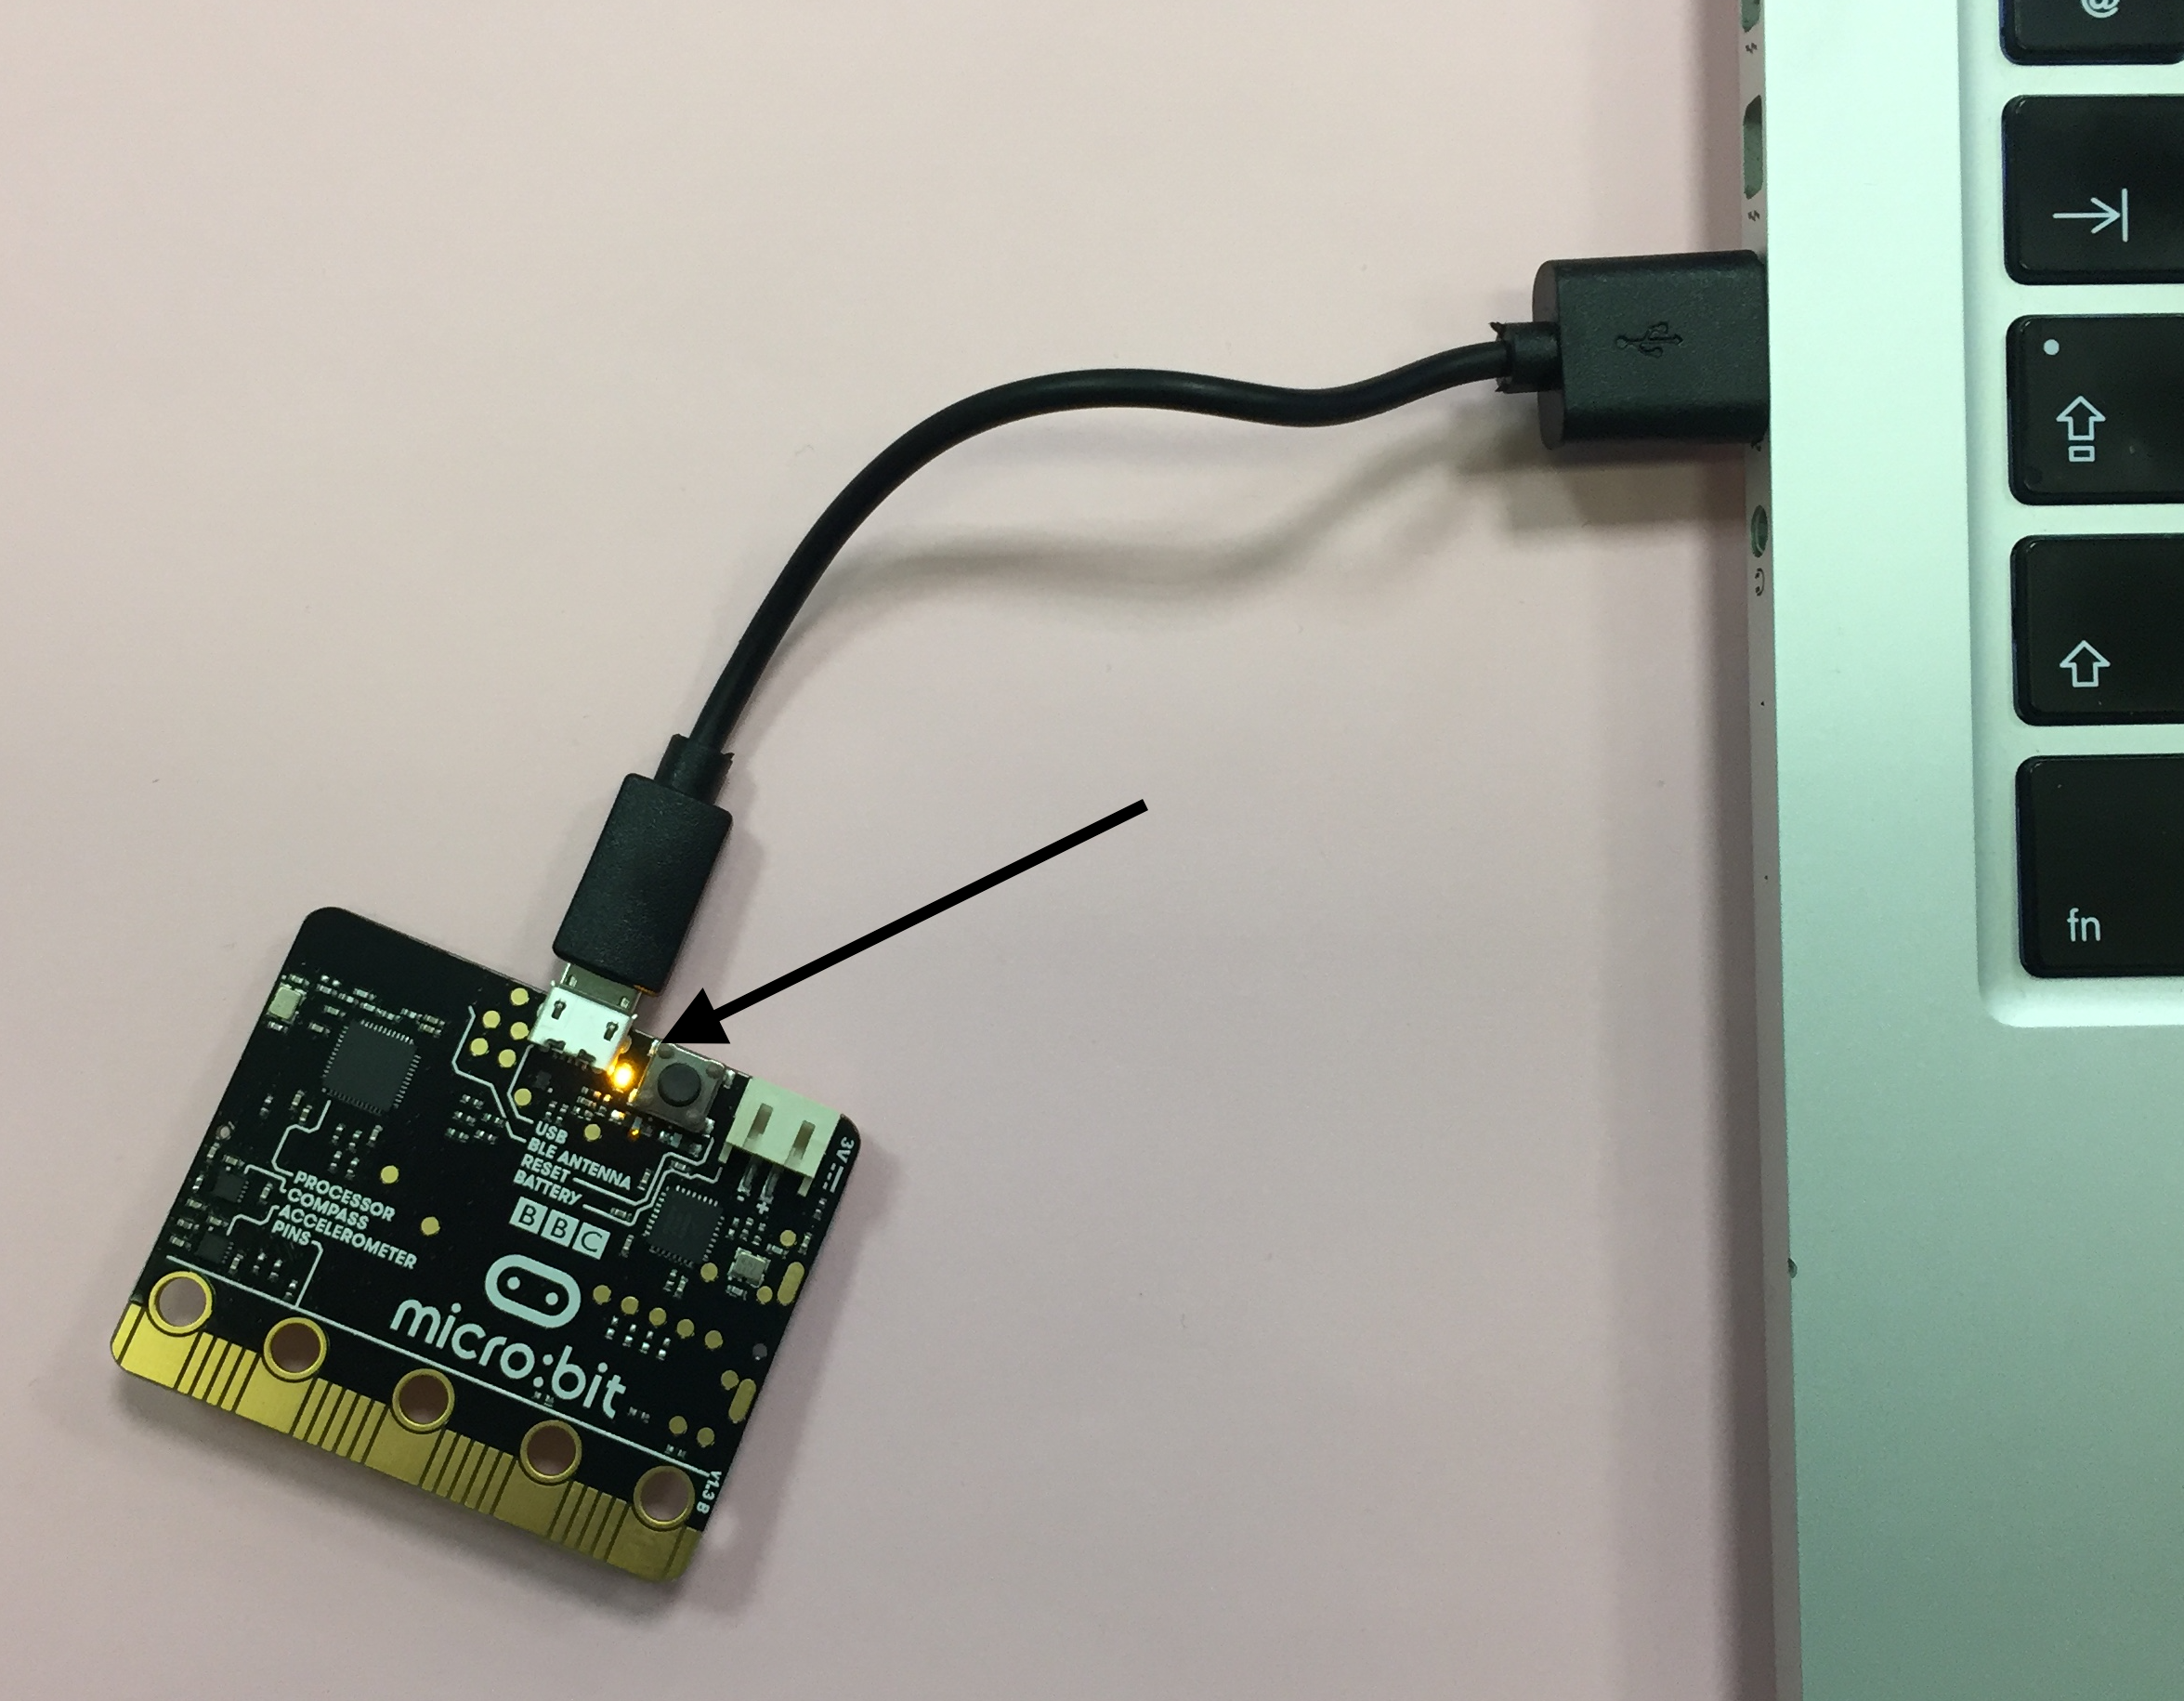
\includegraphics[width=0.45\textwidth]{microbit_telechargement}\\
\end{center}
4 - Enregistrer le fichier compilé (voir la fenêtre "ouverture de \texttt{microbit.hex}" dans l'image ci-dessus), puis le copier dans le répertoire du micro:bit. Un répertoire associé au périphérique usb micro:bit est normalement accessible dans l'explorateur de fichier. Ce répertoire est normalement accessible après avoir connecté la carte au port USB de l'ordinateur. \\
5 - Observer que la lumière jaune (voir la LED pointée dans l'image ci-dessous) clignote jusqu'à ce que le téléchargement du programme sur la carte électronique soit terminé. \\
6 - Observer que le programme marche : des caractères défilent sur la matrice de leds au dos du micro:bit (voir l'image ci-dessous).

\question Quel est la différence entre le code source et le code executable d'un programme ?
\reponse
%
\begin{center}
\includegraphics[width=0.45\textwidth]{microbit_leds}\\
Défilement du texte sur les leds au dos de la carte électronique micro:bit.
\end{center}
%
\question Qu'est ce que "compiler" un programme ?
\reponse

\question Modifier le texte ("Hello world !") par un autre. Quelle ligne de code avez vous modifié ?
\reponse
%}}}

\bigskip

\partie{Bouton}\\ %{{{1
Jusqu'à présent, nous avons créé du code qui permet à l'appareil de faire quelque chose. C'est ce qu'on appelle la sortie . Cependant, nous avons également besoin de l'appareil pour réagir aux choses. De telles choses sont appelées entrées.
\lstset{frame=shadowbox, rulesepcolor=\color{gray}}
\begin{lstlisting}
from microbit import *
sleep(10000)
display.scroll(str(button_a.get_presses()))
\end{lstlisting}

\question Que fait le programme ?
Attendez 10 secondes tout en appuyant 3 fois sur le bouton A. Si besoin, vous pouvez redémarrer le programme en appuyant sur le bouton RESET (indiqué sur la carte).
\reponse

\question Changez 10000 par 2000, testez puis décrivez le résultat.
\reponse

\question Dans quelle unité la valeur 2000 est-elle exprimée ?
\reponse

Entrez maintenant le programme suivant :
\begin{lstlisting}
# ce programme est un test
from microbit import *
sleep(10000)
n = button_a.get_presses()
t = str(n)
display.scroll(t)
\end{lstlisting}

\question Est-ce que le résultat de ce programme est différent ?
\reponse

\question Que fait la ligne \texttt{n = button\_a.get\_presses()} ?
\reponse

\question Que fait la ligne \texttt{t = str(n)} ?\footnote{http://lmgtfy.com/?q=python+str()}
\reponse

\question Que fait la ligne \texttt{display.scroll(t)} ?
\reponse

\question Que faisait donc la ligne display.scroll(str(button\_a.get\_presses())) ?
\reponse

\question Que fait la ligne \texttt{\# ce programme est un test} ? A quoi ça sert ? \footnote{On appelle ce type de ligne un commentaire}
\reponse
%}}}

\bigskip

\partie{Programmer une boucle infinie}\\ %{{{1
\begin{lstlisting}
from microbit import *
while True:
    display.show(Image.HAPPY)
    sleep(2000)
    display.show(Image.SAD)
    sleep(1000)
\end{lstlisting}

\question Décrire ce programme ligne à ligne ?
\reponse

\begin{lstlisting}
from microbit import *
while True:
    display.show(Image.HAPPY)
    sleep(2000)
display.show(Image.SAD)
sleep(1000)
\end{lstlisting}

\question Avec ce nouveau programme, avez-vous une chance voir le visage triste ?
\reponse

\begin{lstlisting}
from microbit import *
while True:
    display.show(Image.HAPPY)
    sleep(2000)
    display.show(Image.SAD)
    sleep(1)
\end{lstlisting}
\question Avec ce nouveau programme, avez-vous une chance voir le visage triste ?
\reponse

\begin{lstlisting}
from microbit import *
while True:
    display.show(Image.HAPPY)
    sleep(2000)
    display.show(Image.SAD)
    sleep(100)
\end{lstlisting}
\question Et maintenant ?
\reponse

\question Quel est le nom de la boucle infinie en anglais ? Quel est le nom de la rue de l'entreprise Apple à Cuppertino ?
\reponse
%}}}

\end{document}
% vim:fdl=0
